\documentclass[11pt]{beamer}
\usetheme{Malmoe}
\usepackage[utf8]{inputenc}
\usepackage{babel}[spanish]
\usepackage{amsmath}
\usepackage{amsfonts}
\usepackage{amssymb}
\usepackage{graphicx}
\usepackage{hyperref}
\usepackage{fancyvrb}
\usepackage{listings}
\usepackage{xcolor}

\author{Diego Alejandro Martinez Jimenez}
\title{Moogle}
%\setbeamercovered{transparent} 
%\setbeamertemplate{navigation symbols}{} 
%\logo{} 
%\institute{} 
%\date{} 
%\subject{} 
\begin{document}

\begin{frame}
\titlepage
\end{frame}

%\begin{frame}
%\tableofcontents
%\end{frame}
\renewcommand{\thesection}{\arabic{section}}

\begin{frame}{Instrucciones para correr el proyecto}

    \textbf{Abrir una terminal en la carpeta del proyecto y escribir lo siguiente:}
    
    \begin{itemize}
        \item Linux:
              \begin{itemize} \item \texttt{make dev} \end{itemize}
        \item Windows:
              \begin{itemize} \item \texttt{dotnet watch run --project MoogleServer}\end{itemize}
    \end{itemize}

\end{frame}

\section*{Introduccion}

\begin{frame}
    
    \frametitle{Introduccion}
    
    Aceptando la mision que se me fue otorgada, ayude en la implementacion de \textbf{Moogle!}. Para ello tuve en cuenta la informacion que me pudieron proporcionar acerca de "\textbf{TF-IDF}" y "\textbf{Algebra lineal}".Tambien me fue util este link \hyperlink{https://en.wikipedia.org/wiki/Tf\%E2\%80\%93idf}{\textcolor{blue}{TF-IDF}}.
    
    
\end{frame}

\begin{frame}[fragile]
    \frametitle{Arquitectura del proyecto}
    \begin{figure}[h]
        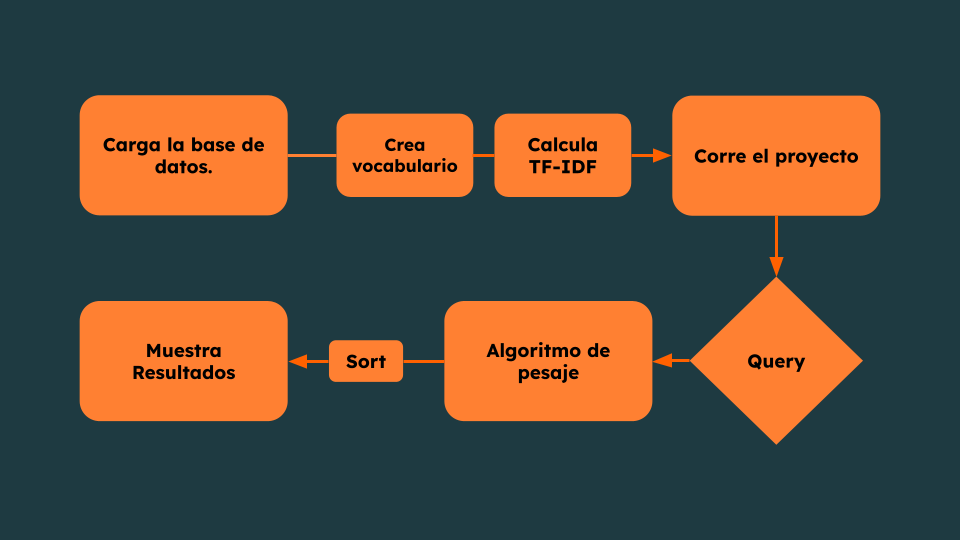
\includegraphics[width = 1\linewidth]{Project.png}
        \caption{Orden de los procesos del proyecto.}
    \end{figure}
\end{frame}

\section*{Cargando la base Datos}
\begin{frame}[fragile]
    \frametitle{Cargando la base de Datos}
    Lo primero que implemente fue una clase que nombre \texttt{Documents} esta contiene varios metodos relacionados con operaciones que se le pueden a hacer a documentos, por ejemplo el metodo \texttt{Documents.ReadText()} el cual retorna como string toda el texto de un .txt. Lo mas importante de esta clase es su constructor.
    \begin{small}
    \end{small}
\end{frame}

\begin{frame}[fragile]
    \frametitle{La clase Documents}
    Este recibe como parametro \texttt{string path} que debera ser un string con la direccion de una carpeta donde esten almacenados documentos \emph{.txt}, \textit{(de no ser asi no garantizo su correcto funcionamiento)}. 
    \begin{Verbatim}[frame=single]
public Documents(string path){
    this.path = path
    this.directory = GetDocuments(this.path);
    this.Vocabulary = GetVocabulary();
    foreach(string file in this.directory)
    documents++;
    
    this.documents = documents;
    this.ComputeDocuments();
}
    \end{Verbatim}
    
\end{frame}

\begin{frame}
    \frametitle{TF-IDF}
    \begin{flushleft}
        
        Al crear una instancia de \texttt{Documents} esta asigna un numero a cada termino encontrado en el corpus, (el metodo encargado de este proceso es \texttt{Documents.GetVocabulary}) luego el metodo \texttt{ComputeDocuments()} calcula el TF-IDF de cada documento, creando una matriz donde \texttt{TFIDF[i,j]} tiene guardado el TF-IDF de el termino j en el documento i. Toda la informacion util es almacenada en variables tipo \texttt{static} para su uso posterior.\\
        \vspace{5pt}
        La formula usada para calcular el TF - IDF es la siguiente:
        
        %TF-IDF formulas
        \begin{center}
            
            $    
            % \mathrm{tf}(t,d) = \frac{f_{t,d}}{\max\{f_{t',d}:t' \in d\}}\linebreak\linebreak
            % \mathrm{idf}(t,D) = \log \frac{N}{|\{d \in D: t \in d\}|}\linebreak\linebreak
            \mathrm{TF\text{-}IDF}(i,j,D) = \mathrm{TF}(i,D) \cdot \mathrm{IDF}(i,j)
            $
        
        \end{center}

    Donde \emph{ \text{D} } seria el corpus donde se calcula el TF-IDF.
\end{flushleft}

\end{frame}

\begin{frame}[fragile]
    \frametitle{Vectores y Matrices}
    En las clases \texttt{Algebra.Vector} y \texttt{Algebra.Matrix} estan implementados en metodos las operaciones relacionadas con estos conceptos provenientes del \textbf{Algebra Lineal}. Estas son fundamentales para el funcioanmiento de \texttt{MoogleEngine.Documents}.
    \vspace{5pt}
    Ejemplos de metodos en estas clases:
    \begin{Verbatim}[frame=single]
public static double DotProduct(Vector A, Vector B){     
    double result = 0;

    for(int i = 0; i < A.count; i++){
        result += A[i]*B[i];
    }
        
    return result;
}
    \end{Verbatim}
   
\end{frame}

\section{Respondiendo la Query}
\begin{frame}
    \frametitle{Respondiendo la Query}

    Luego de implementar estas clases, arregle la clase Moogle la cual en su momento no era muy util. El objetivo principal de esta clase es responder a la query a traves del metodo \texttt{Moogle.Query}. La idea para este metodo es modelar un vector en el que cada componente de este, sea el TF-IDF de cada termino que pertenezca al corpus de documentos. Luego hallar el coseno entre este vector y cada uno de los vectores creados a partir de los documentos.
    
\end{frame}

\begin{frame}[fragile]
    \frametitle{Respondiendo la Query}
    
    Primero guardo en variables el TF-IDF, el IDF y el vocabulario previamentes calculados al cargar los documentos.
    
    \begin{Verbatim}[frame=single,fontsize=\small]
Matrix TFIDF = Documents._TFIDF;
Vector idf = Documents._IDF;
Dictionary<string,int> vocabulary = Documents._Vocabulary;
        
    \end{Verbatim}
\end{frame}

\begin{frame}[fragile]
    \frametitle{Calculo del TF-IDF}

    Luego calcula el TF-IDF de cada termino en la query, en caso de un termino de la query no encontrarse en vocabulary sera ignorado:

    \begin{Verbatim}[frame=single]
tfidf = Documents.CalculateTF(query,vocabulary);

for(int i = 0; i < idf.Count; i++){
    tfidf[i] *= idf[i];
}
\end{Verbatim}
\end{frame}
\begin{frame}[fragile]
    \frametitle{El score}
    El \emph{Producto Punto} se calcula con el metodo \texttt{Vector.DotProduct} que hace pues exactamente lo que su nombre indica. Luego el resultado del calculo sera el score de su respectivo documento. Luego los documentos son ordenados con el metodo \texttt{Array.Sort} dependiendo de su respectivo score. En caso de que el score de un documento sea 0 es ignorado pues no tiene relevancia alguna con la query.\linebreak\\
    Luego se construye un \texttt{SearchResult} a partir de esta informacion guardada en \texttt{items}.\\
\begin{Verbatim}[frame=single]
return new SearchResult(items, suggestion);
\end{Verbatim}
\end{frame}

\subsection{Las sugerencias}

\begin{frame}[fragile]
    \frametitle{Las Sugerencias}
    
    Para las sugerencias use el algoritmo de \href{https://es.wikipedia.org/wiki/Distancia_de_Levenshtein}{\textcolor{blue}{Distancia de Levenshtein}}. Este calcula de forma dinamica el número mínimo de operaciones requeridas para transformar una cadena de caracteres en otra. El metodo para esto es \texttt{Documents.EditDistance}.\linebreak

    Al recibir una query la sugerencia se calcula dentro del metodo \texttt{Utils.Suggestion} que por cada termino guardado en vocabulary calcula su respectiva Distancia de Levenshtein con respecto a la query.\linebreak

    En caso de que no se encuentre ningun termino relacionado con query, \texttt{Moogle.Query} retornara los documentos relacionados con la sugerencia.
\end{frame}


\end{document}